\documentclass[../main.tex]{subfiles}
\setlength{\columnsep}{4pt}
\begin{document}
\noindent{Angels are a race of celestials, beings who live on the good-aligned Outer Planes. Celestials positively drip with goodness--every fiber of their bodies and souls is suffused with it. They are the natural enemies of demons and devils (creatures of the infernal realms)}\\
\indent{Angels can be of any good alignment. Lawful good angels hail from the plane of Celestia, neutral good angels from the plane of Elysium or the Beastlands, and Chaotic good angels from the plane of Arborea. Regardless of their alignment, angels never lie, cheat, or steal. They are impeccably honorable in all their dealings and often prove the most trustworthy and diplomatic of all the celestials.}\\
\indent{All angels are blessed with comely looks, though their actual appearances vary widely.}\\
\indent{Angels speak Celestial, Infernal, and Draconic, though they can speak with almost any creature because of their tongues ability.}\\
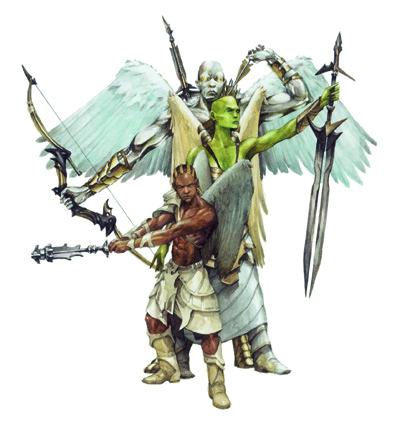
\includegraphics[width=\columnwidth]{Angel}
\dndsection{COMBAT}
\noindent{Though they are honorable, and good, angels don't hesitate to back up their arguments with their weapons and other powers when necessary. Though they do not relish combat, they do not hesitate to take the battle to the enemy. In combat, most angels make full use of their mobility and their ability to attack at a distance.}\\
\indent{\textbf{Angel Traits:} An angel possesses the following traits (unless otherwise noted in a creature?s entry).}\\
\indent{--Darkvision out to 60 feet and low-light vision.}\\
\indent{--Immunity to acid, cold, and petrification.}\\
\indent{--Resistance to electricity 10 and fire 10.}\\
\indent{ +4 racial bonus on saves against poison.}\\
\indent{--\textit{Protective Aura (Su):} Against attacks made or effects created by evil creatures, this ability provides a +4 deflection bonus to AC and a +4 resistance bonus on saving throws to anyone within 20 feet of the angel. Otherwise, it functions as a \textit{magic circle against evil} effect and a \textit{lesser globe of invulnerability}, both with a radius of 20 feet (caster level equals angel?s HD). This aura can be dispelled, but the angel can create it again as a free action on its next turn. (The defensive benefits from the circle are not included in an angel?s statistics block.)}\\
\indent{--\textit{Tongues (Su):} All angels can speak with any creature that has a language, as though using a \textit{tongues} spell (caster level equal to angel?s Hit Dice). This ability is always active.}\\
\clearpage

\dndsection{ANGEL, ASTRAL DEVA}\vspace{-4mm}
\begin{table}[H]
\centering
\resizebox{\columnwidth}{!}{%
\begin{tabular}{lp{16em}}
 & \textbf{Medium Outsider (Angel, Extraplanar, Good)} \\
\textbf{Hit Dice:} & 12d8+48 (102 hp) \\
\textbf{Initiative:} & +8 \\
\textbf{Speed:} & 50 ft. (10 squares), fly 100 ft. (good) \\
\textbf{Armor Class:} & 29 (+4 Dex, +15 natural), touch 14, flat-footed 25 \\
\textbf{Base Attack/Grapple:} & +12/+18 \\
\textbf{Attack:} & +3 heavy mace of disruption +21 melee (1d8+12 plus stun) or slam +18 melee (1d8+9) \\
\textbf{Full Attack:} & +3 heavy mace of disruption +21/+16/+11 melee (1d8+12 plus stun) or slam +18 melee (1d8+9) \\
\textbf{Space/Reach:} & 5 ft./5 ft. \\
\textbf{Special Attacks:} & Spell-like abilities, stun \\
\textbf{Special Qualities:} & Damage reduction 10/evil, darkvision 60 ft., low-light vision, immunity to acid, cold, and petrification, protective aura, resistance to electricity 10 and fire 10, spell resistance 30, tongues, uncanny dodge \\
\textbf{Saves:} & Fort +14 (+18 against poison), Ref +12, Will +12 \\
\textbf{Abilities:} & Str 22, Dex 18, Con 18, Int 18, Wis 18, Cha 20 \\
\textbf{Skills:} & Concentration +19, Craft or Knowledge (any three) +19, Diplomacy +22, Escape Artist +19, Hide +19, Intimidate +20, Listen +23, Move Silently +19, Sense Motive +19, Spot +23, Use Rope +4 (+6 with bindings) \\
\textbf{Feats:} & Alertness, Cleave, Great Fortitude, Improved Initiative, Power Attack \\
\textbf{Environment:} & Any good-aligned plane \\
\textbf{Organization:} & Solitary, pair, or squad (3?5) \\
\textbf{Challenge Rating:} & 14 \\
\textbf{Treasure:} & No coins; double goods; standard items \\
\textbf{Alignment:} & Always good (any) \\
\textbf{Advancement:} & 13?18 HD (Medium); 19?36 HD (Large) \\
\textbf{Level Adjustment:} & +8 \\
\end{tabular}%
}
\end{table}

\noindent{\textit{A beautiful, extremely tall, humanlike creature with long, feathery wings and a very supple and lithe body glows with an inner power that makes it hard to look directly at the creature}}

\noindent{Astral devas watch over lesser beings of good alignment and help when they can. In particular, they are patrons of planar travellers and powerful creatures undertaking good causes.}
\indent{An astral deva is about 7-\textonehalf\ feet tall and weighs about 250 pounds.}

\dndsubsection{Combat}
\noindent{An astral deva is not afraid to enter melee combat. It takes a fierce joy in bashing evil foes with its powerful \textit{+3 heavy mace of disruption.}}\\
\indent{An astral deva's natural weapons, as well as any weapons it wields, are treated as good-aligned for the purpose of overcoming damage reduction.}\\
\indent{\textbf{Spell-Like Abilities:} At will--\textit{aid}, \textit{continual flame}, \textit{detect evil}, \textit{discern lies} (DC 19), \textit{dispel evil} (DC 20), \textit{dispel magic}, \textit{holy aura} (DC 23), \textit{holy smite} (DC 19), \textit{holy word} (DC 22), \textit{invisibility} (self only), \textit{plane shift} (DC 22), \textit{polymorph} (self only), r\textit{emove curse} (DC 18), \textit{remove disease} (DC 18), \textit{remove fear} (DC 16); 7/day--\textit{cure light wounds} (DC 16), \textit{see invisibility}; 1/day--\textit{blade barrier} (DC 21), \textit{heal} (DC 21). Caster level 12th. The save DCs are Charisma-based.}\\
\indent{\textbf{Stun (Su):} If an astral deva strikes an opponent twice in one round with its mace, that creature must succeed on a DC 22 Fortitude save or be stunned for 1d6 rounds. The save DC is Strength-based.}\\
\indent{\textbf{Uncanny Dodge (Ex):} An astral deva retains its Dexterity bonus to AC when flat-footed, and it cannot be flanked except by a rogue of at least 16th level. It can flank characters with the uncanny dodge ability as if it were a 12th-level rogue.}\\
\clearpage

\dndsection{ANGEL, PLANETAR}\vspace{-4mm}
\begin{table}[H]
\centering
\resizebox{\columnwidth}{!}{%
\begin{tabular}{lp{16em}}
 & \textbf{Large Outsider (Angel, Extraplanar, Good)} \\
\textbf{Hit Dice:} & 14d8+70 (133 hp) \\
\textbf{Initiative:} & +8 \\
\textbf{Speed:} & 30 ft. (6 squares), fly 90 ft. (good) \\
\textbf{Armor Class:} & 32 (?1 size, +4 Dex, +19 natural), touch 13, flat-footed 28 \\
\textbf{Base Attack/Grapple:} & +14/+25 \\
\textbf{Attack:} & +3 greatsword +23 melee (3d6+13/19?20) or slam +20 melee (2d8+10) \\
\textbf{Full Attack:} & +3 greatsword +23/+18/+13 melee (3d6+13/19?20) or slam +20 melee (2d8+10) \\
\textbf{Space/Reach:} & 10 ft./10 ft. \\
\textbf{Special Attacks:} & Spell-like abilities, spells \\
\textbf{Special Qualities:} & Damage reduction 10/evil, darkvision 60 ft., low-light vision, immunity to acid, cold, and petrification, protective aura, regeneration 10, resistance to electricity 10 and fire 10, spell resistance 30, tongues \\
\textbf{Saves:} & Fort +14 (+18 against poison), Ref +13, Will +15 \\
\textbf{Abilities:} & Str 25, Dex 19, Con 20, Int 22, Wis 23, Cha 22 \\
\textbf{Skills:} & Concentration +22, Craft or Knowledge (any four) +23, Diplomacy +25, Escape Artist +21, Hide +17, Intimidate +23, Listen +23, Move Silently +21, Sense Motive +23, Search +23, Spot +23, Use Rope +4 (+6 with bindings) \\
\textbf{Feats:} & Blind-Fight, Cleave, Improved Initiative, Improved Sunder, Power Attack \\
\textbf{Environment:} & Any good-aligned plane \\
\textbf{Organization:} & Solitary or pair \\
\textbf{Challenge Rating:} & 16 \\
\textbf{Treasure:} & No coins; double goods; standard items \\
\textbf{Alignment:} & Always good (any) \\
\textbf{Advancement:} & 15?21 HD (Large); 22?42 HD (Huge) \\
\textbf{Level Adjustment:} & -- \\
\end{tabular}%
}
\end{table}

\noindent{\textit{The creature resembles a massively muscular and tall human with smooth emerald skin, white-feathered wings, and a bald head.}}\\

\noindent{Planetars serve as mighty generals of celstial armies. They also help powerful mortals on missions of good, particularly those that involve battles with fiends. A planetar is nearly 9 feet tall and weighs about 500 pounds.}\\

\dndsubsection{Combat}
\noindent{Despite their vast array of magical powers, planetars are likely to wade into melee with their +3 greatswords. They particularly enjoy fighting fiends.}\\
\indent{A planetar?s natural weapons, as well as any weapons it wields, are treated as good-aligned for the purpose of overcoming damage reduction.}\\
\indent{\textbf{Regeneration:} A planetar takes damage from evil-aligned weapons and from spells and effects with the evil descriptor.}\\
\indent{\textbf{Spell-Like Abilities:} At will--\textit{continual flame}, \textit{dispel magic}, \textit{holy smite} (DC 20), \textit{invisibility} (self only), \textit{lesser restoration} (DC 18), \textit{remove curse} (DC 19), \textit{remove disease} (DC 19), \textit{remove fear} (DC 17), \textit{speak with dead} (DC 19); 3/day--\textit{blade barrier} (DC 22), \textit{flame strike} (DC 21), \textit{polymorph} (self only), \textit{power word stun}, \textit{raise dead}, \textit{waves of fatigue}; 1/day--\textit{earthquake} (DC 24), \textit{greater restoration} (DC 23), \textit{mass charm monster} (DC 24), \textit{waves of exhaustion}. Caster level 17th. The save DCs are Charisma-based.}\\
\indent{The following abilities are always active on the planetar?s person, as the spells (caster level 17th): \textit{detect evil}, \textit{detect snares and pits}, \textit{discern lies} (DC 20), \textit{see invisibility}, and \textit{true seeing}. They can be dispelled, but the planetar can reactivate them as a free action.}\\
\indent{\textbf{Spells:} Planetars can cast divine spells as 17th-level clerics. A planetar has access to two of the following domains: Air, Destruction, Good, Law, or War (plus any others from its deity). The save DCs are Wisdom-based.}\\
\noindent{\textit{Typical Cleric Spells Prepared} (6/8/8/7/7/6/6/4/3/2; save DC 16 + spell level): 0--\textit{create water}, \textit{detect magic}, \textit{guidance}, \textit{resistance} (2), \textit{virtue}; 1st--\textit{bless} (2), \textit{cause fear}, \textit{divine favor} (2), \textit{entropic shield}, \textit{inflict light wounds*}, \textit{shield of faith}; 2nd--\textit{aid*}, \textit{align weapon}, \textit{bear ?s endurance}, \textit{bull?s strength} (2), \textit{consecrate, eagle?s splendor}, \textit{hold person}; 3rd--\textit{contagion*}, \textit{daylight}, \textit{invisibility purge}, \textit{prayer} (2), \textit{summon monster III}, \textit{wind wall}; 4th--\textit{death ward}, \textit{dismissal}, \textit{inflict critical wounds*}, \textit{neutralize poison} (2), \textit{summon monster IV}; 5th--\textit{break enchantment}, \textit{circle of doom*}, \textit{dispel evil}, \textit{mark of justice}, \textit{plane shift}, \textit{righteous might}; 6th--\textit{banishment}, \textit{greater dispel magic}, \textit{harm*}, \textit{heal}, \textit{heroes? feast}, \textit{mass cure moderate wounds}; 7th--\textit{dictum}, \textit{disintegrate*}, \textit{holy word}, \textit{regenerate}; 8th--\textit{holy aura*}, \textit{mass cure critical wounds}, \textit{shield of law}; 9th--\textit{implosion}, \textit{summon monster IX (good)*}.}\\
\noindent{*Domain spell. Domains: Destruction and Good.}
\clearpage

\dndsection{ANGEL, SOLAR}\vspace{-4mm}
\begin{table}[H]
\centering
\resizebox{\columnwidth}{!}{%
\begin{tabular}{lp{16em}}
 & \textbf{Large Outsider (Angel, Extraplanar, Good)} \\
\textbf{Hit Dice:} & 22d8+110 (209 hp) \\
\textbf{Initiative:} & +9 \\
\textbf{Speed:} & 50 ft. (10 squares), fly 150 ft. (good) \\
\textbf{Armor Class:} & 35 (?1 size, +5 Dex, +21 natural), touch 14, flat-footed 30 \\
\textbf{Base Attack/Grapple:} & +22/+35 \\
\textbf{Attack:} & +5 dancing greatsword +35 melee (3d6+18/19?20) or +2 composite longbow (+5 Str bonus) +28 ranged (2d6+7/x3 plus slaying) or slam +30 melee (2d8+13) \\
\textbf{Full Attack:} & +5 dancing greatsword +35/+30/+25/+20 melee (3d6+18/19?20) or +2 composite longbow (+5 Str bonus) +28/+23/+18/+13 ranged (2d6+7/x3 plus slaying) or slam +30 melee (2d8+13) \\
\textbf{Space/Reach:} & 10 ft./10 ft. \\
\textbf{Special Attacks:} & Spell-like abilities, spells \\
\textbf{Special Qualities:} & Damage reduction 15/epic and evil, darkvision 60 ft., low-light vision, immunity to acid, cold, and petrification, protective aura, regeneration 15, resistance to electricity 10 and fire 10, spell resistance 32, tongues \\
\textbf{Saves:} & Fort +18 (+22 against poison), Ref +18, Will +20 \\
\textbf{Abilities:} & Str 28, Dex 20, Con 20, Int 23, Wis 25, Cha 25 \\
\textbf{Skills:} & Concentration +30, Craft or Knowledge (any five) +33, Diplomacy +34, Escape Artist +30, Hide +26, Listen +32, Move Silently +30, Search +31, Sense Motive +32, Spellcraft +31, Spot +32, Survival +7 (+9 following tracks), Use Rope +5 (+7 with bindings) \\
\textbf{Feats:} & Cleave, Dodge, Great Cleave, Improved Initiative, Improved Sunder, Mobility, Power Attack, Track \\
\textbf{Environment:} & Any good-aligned plane \\
\textbf{Organization:} & Solitary or pair \\
\textbf{Challenge Rating:} & 23 \\
\textbf{Treasure:} & No coins; double goods; standard items \\
\textbf{Alignment:} & Always good (any) \\
\textbf{Advancement:} & 23?33 HD (Large); 34?66 HD (Huge) \\
\textbf{Level Adjustment:} & -- \\
\end{tabular}}
\end{table}

\noindent{\textit{The creature resembles a towering, powerfully built human with brilliant topaz eyes, silvery (or golden) skin, and gleaming white wings}}\\

\noindent{Solars are the greatest of the angels, usually close attendants to a deity or champions of cosmically beneficent task (such as eliminating a particular type of wrongdoing).}
\indent{A solar has a deep and commanding voice, and stands about 9 feet tall. It weighs about 500 pounds.}

\dndsubsection{Combat}
\noindent{Solars are puissant champions of good. Only the most powerful fiends approach their power.}\\
\indent{Even more fearsome than their /textit{+5 dancing greatswords} are their /textit{+2 composite longbows} that create any sort of \textit{slaying arrow} when drawn.}\\
\indent{A solar?s natural weapons, as well as any weapons it wields, are treated as good-aligned and epic for the purpose of overcoming damage reduction.}\\
\indent{\textbf{Regeneration (Ex):} A solar takes normal damage from epic evil-aligned weapons, and from spells or effects with the evil descriptor.}\\
\indent{\textbf{Spell-Like Abilities:} At will--\textit{aid}, \textit{animate objects}, \textit{commune}, \textit{continual flame}, \textit{dimensional anchor}, \textit{greater dispel magic}, \textit{holy smite} (DC 21), \textit{imprisonment} (DC 26), \textit{invisibility} (self only), \textit{lesser restoration} (DC 19), \textit{polymorph} (self only), \textit{power word stun}, \textit{remove curse} (DC 20), \textit{remove disease} (DC 20), \textit{remove fear} (DC 18), \textit{resist energy}, \textit{summon monster VII}, \textit{speak with dead} (DC 20), \textit{waves of fatigue}; 3/day--\textit{blade barrier} (DC 23), \textit{earthquake} (DC 25), \textit{heal} (DC 23), \textit{mass charm monster} (DC 25), \textit{permanency}, \textit{resurrection}, \textit{waves of exhaustion}; 1/day--\textit{greater restoration} (DC 24), \textit{power word blind}, \textit{power word kill}, \textit{power word stun}, \textit{prismatic spray} (DC 24), \textit{wish}. Caster level 20th. The save DCs are Charisma-based.}\\
\noindent{The following abilities are always active on a solar?s person, as the spells (caster level 20th): \textit{detect evil}, \textit{detect snares and pits}, \textit{discern lies} (DC 21), \textit{see invisibility}, \textit{true seeing}. They can be dispelled, but the solar can reactivate them as a free action.}\\
\indent{\textbf{Spells:} Solars can cast divine spells as 20th-level clerics. A solar has access to two of the following domains: Air, Destruction, Good, Law, or War (plus any others from its deity). The save DCs are Wisdom-based.}\\
\indent{\textit{Typical Cleric Spells Prepared} (6/8/8/8/7/7/6/6/5/5; save DC 17 + spell level): 0--\textit{create water}, \textit{detect magic}, \textit{guidance} (2), \textit{resistance}  (2); 1st--\textit{bless} (2), \textit{cause fear}, \textit{divine favor} (2), \textit{entropic shield}, \textit{obscuring mist*}, \textit{shield of faith}; 2nd--\textit{align weapon}, \textit{bear?s endurance} (2), \textit{bull?s strength} (2), \textit{consecrate}, \textit{eagle?s splendor}, \textit{spiritual weapon*}; 3rd--\textit{daylight}, \textit{invisibility purge}, \textit{magic circle against evil}, \textit{magic vestment*}, \textit{prayer} (2), \textit{protection from energy}, \textit{wind wall}; 4th--\textit{death ward} (2), \textit{dismissal} (2), \textit{divine power*}, \textit{neutralize poison} (2); 5th--\textit{break enchantment}, \textit{control winds*}, \textit{dispel evil}, \textit{plane shift}, \textit{righteous might} (2), \textit{symbol of pain}; 6th--\textit{banishment}, \textit{chain lightning*}, \textit{heroes? feast}, \textit{mass cure moderate wounds}, \textit{undeath to death}, \textit{word of recall}; 7th--\textit{control weather*}, \textit{destruction}, \textit{dictum}, \textit{ethereal jaunt}, \textit{holy word}, \textit{regenerate}; 8th--\textit{fire storm}, \textit{holy aura}, \textit{mass cure critical wounds} (2), \textit{whirlwind*}; 9th--\textit{etherealness}, \textit{elemental swarm (air)*}, \textit{mass heal}, \textit{miracle}, \textit{storm of vengeance.}}\\
\noindent{*Domain spell. Domains: Air and War.}

\end{document}
